\section{Large language models (LLMs)}

\subsection{Introduction}

Language modeling is a long-standing research topic, dating back to the 1950s with Shnnon's application of information theory to human language, where he measures how well simple n-gram language models predict or compress natural language text \cite{6773263}. Since then, statistical language modeling became fundamental to many natural language understanding and generation tasks, ranging from speech recognition, machine translation, to information retrieval \cite{Jelinek1997StatisticalMF} \cite{Manning_Raghavan_Schütze_2008}.

Recent advances in transformer-based large language models (LLMs), pretrained on web-scale text corpora, have significantly enhanced the capabilities of these models. For instance, OpenAI's ChatGPT and GPT-4 are now used not only for natural language processing but also as general task solvers, exemplified by their integration into Microsoft's Co-Pilot systems. These models can follow complex human instructions and perform multi-step reasoning when necessary. Consequently, LLMs are becoming fundamental building blocks for the development of general-purpose AI agents or artificial general intelligence (AGI).

LLMs are large-scale, pre-trained, statistical language models based on neural networks. Their recent success is the result of decades of research and development in language modeling, which can be divided into four distinct waves, each with its own starting points and progression: statistical language models, neural language models, pre-trained language models, and LLMs.

Early neural language models (NLMs) \cite{NIPS2000_728f206c}, \cite{schwenk-etal-2006-continuous}, \cite{mikolov10_interspeech}, \cite{graves2014generating} address data sparsity by mapping words to low-dimensional continuous vectors, known as embedding vectors, and predicting the next word based on the aggregation of these vectors using neural networks. The embedding vectors learned by NLMs create a hidden space where the semantic similarity between vectors can be easily computed as their distance. This enables the computation of semantic similarity between any two inputs, regardless of their forms (e.g., queries versus documents in web search \cite{10.1145/2505515.2505665}, \cite{gao2022neural}, sentences in different languages in machine translation \cite{sutskever2014sequence}, \cite{cho2014properties}) or modalities (e.g., image and text in image captioning \cite{cho2014properties}, \cite{vinyals2015tell}). However, early NLMs are task-specific models, as they are trained on task-specific data, resulting in a hidden space that is also task-specific.

Pre-trained language models (PLMs), unlike early neural language models (NLMs), are task-agnostic. This generality also extends to the learned hidden embedding space. The training and inference of PLMs follow the pre-training and fine-tuning paradigm, where language models utilizing recurrent neural networks \cite{peters2018deep} or transformers \cite{devlin2019bert}, \cite{liu2019roberta}, \cite{he2021deberta} are pre-trained on web-scale unlabeled text corpora for general tasks such as word prediction. They are then fine-tuned for specific tasks using small amounts of labeled, task-specific data. Recent surveys on PLMs include \cite{zhou2023comprehensive}, \cite{han2021pretrained}, \cite{Qiu_2020}.

Large language models (LLMs) mainly refer to transformer-based neural language models that contain tens to hundreds of billions of parameters. These models, such as PaLM \cite{chowdhery2022palm}, LLaMA \cite{touvron2023llama}, and GPT-4 \cite{openai2024gpt4}, are pre-trained on massive text datasets. Compared to pre-trained language models (PLMs), LLMs are not only significantly larger in model size but also exhibit stronger language understanding and generation abilities. More importantly, they demonstrate emergent abilities not present in smaller-scale language models. As illustrated in Figure \ref{fig:llm-capabilities}, these emergent abilities include:

\textbf{In-context learning}: LLMs can learn a new task from a small set of examples presented in the prompt at inference time.

\textbf{Instruction following}: After instruction tuning, LLMs can follow instructions for new types of tasks without explicit examples.

\textbf{Multi-step reasoning}: LLMs can solve complex tasks by breaking them down into intermediate reasoning steps, as demonstrated in the chain-of-thought prompting \cite{wei2023chainofthought}.

LLMs can also be augmented with external knowledge and tools \cite{mialon2023augmented}, \cite{mialon2023augmented}, enabling them to effectively interact with users and the environment \cite{mialon2023augmented}, and continually improve using feedback data collected through interactions, such as via reinforcement learning with human feedback (RLHF).

\begin{figure}[H]
    \centering
    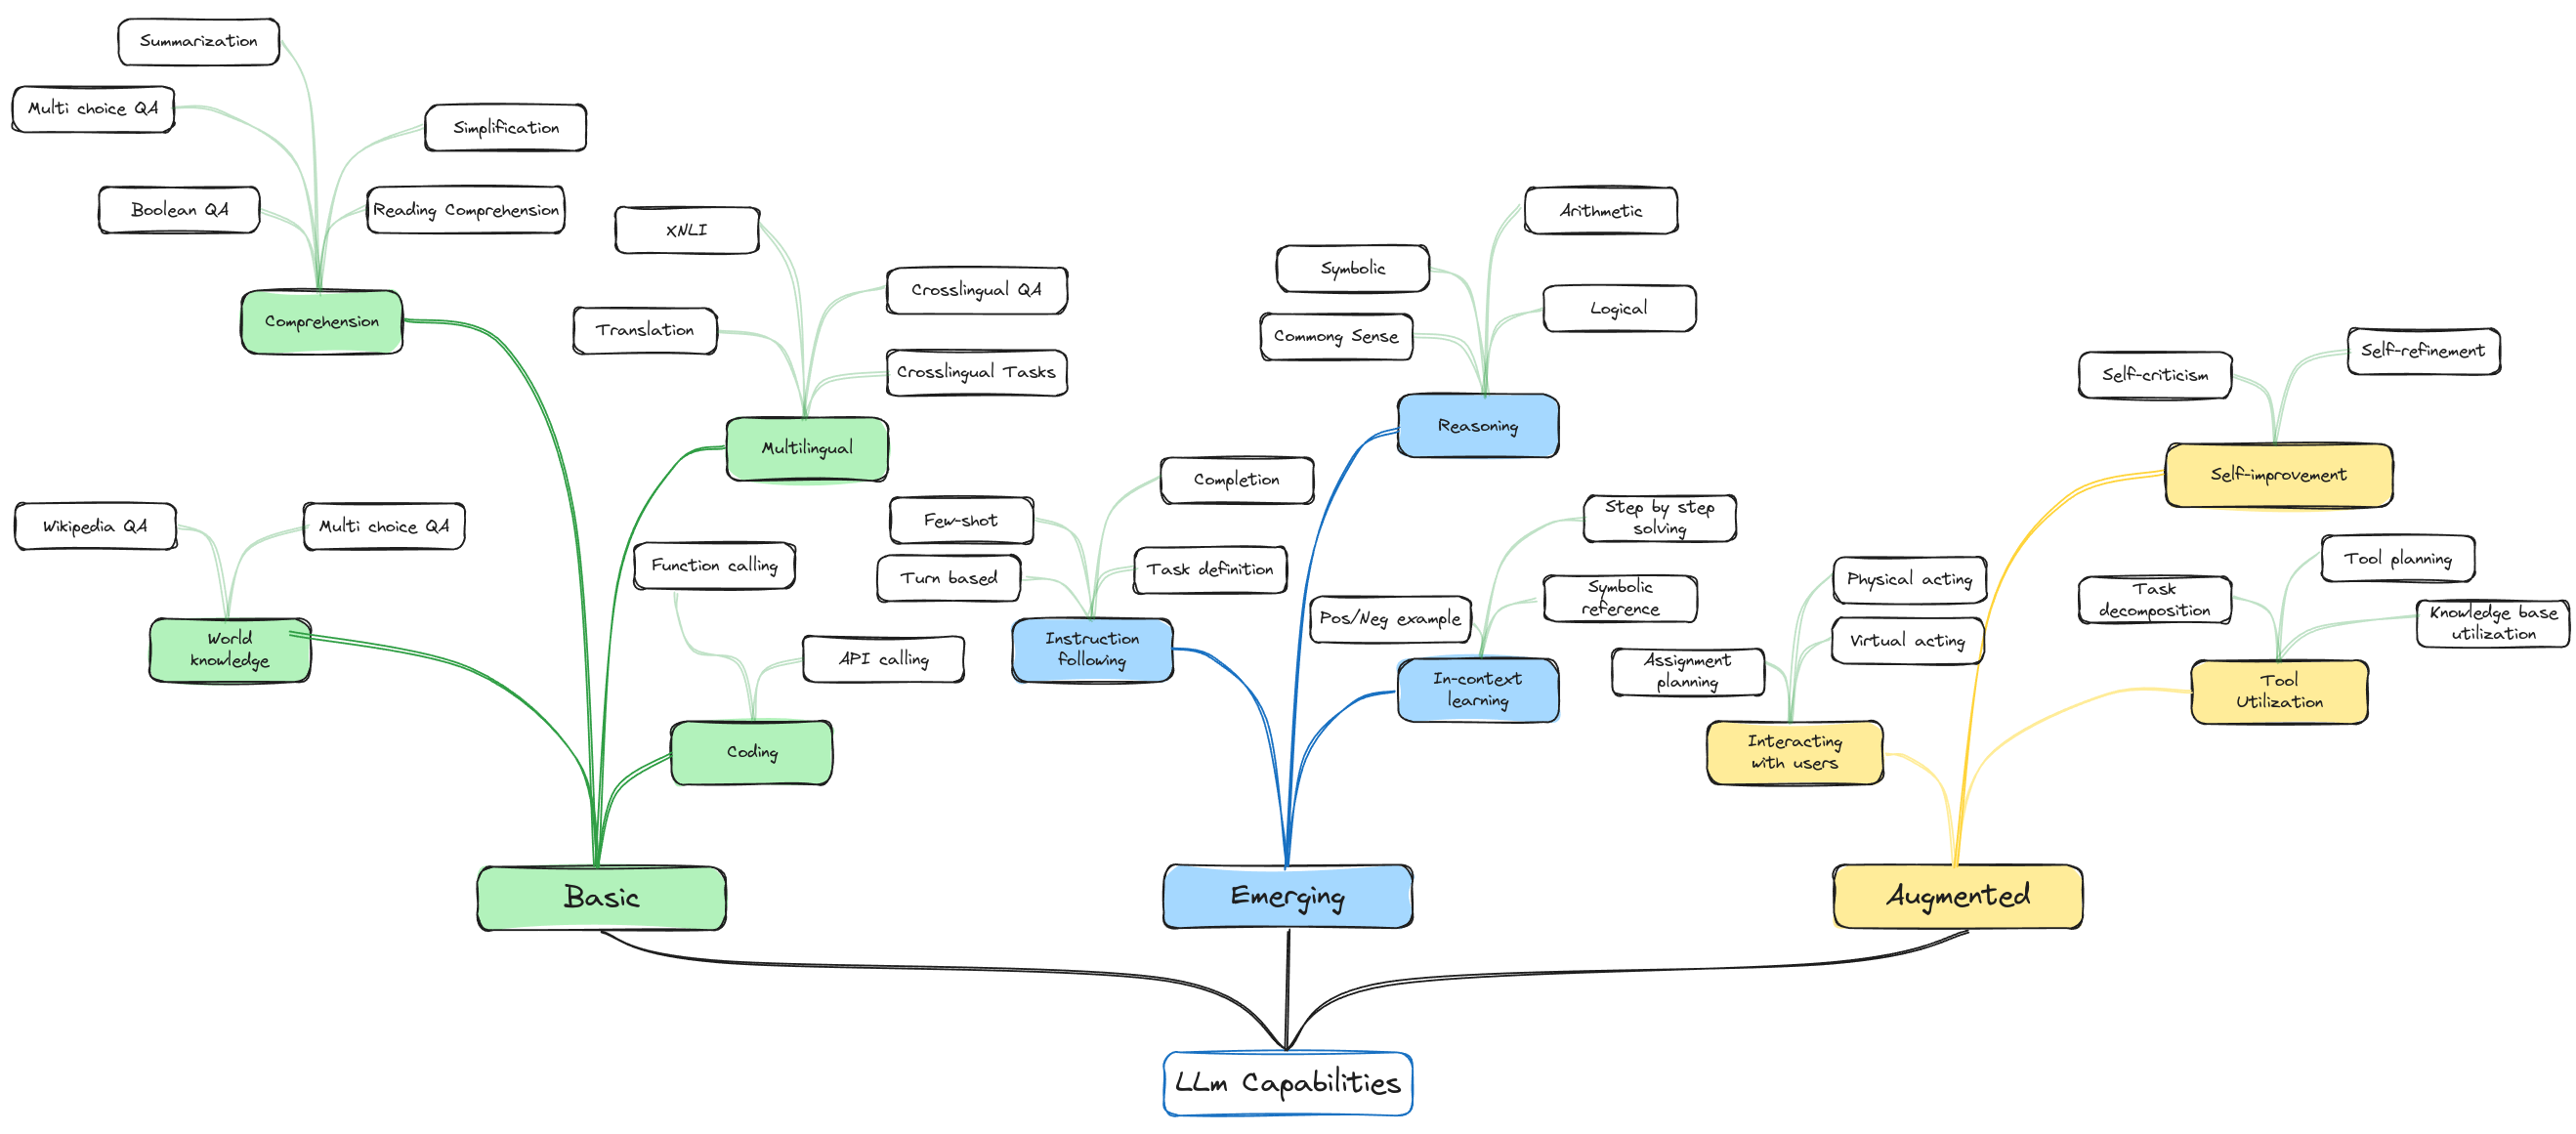
\includegraphics[width=\textwidth,height=6cm,keepaspectratio=true]{llm-capabilities.png}
    \caption{
        \it{LLM capabilities \cite{minaee2024large}}
    }
    \label{fig:llm-capabilities}
\end{figure}

\subsection{Large Language Model Families}

Large language models (LLMs) primarily refer to transformer-based pre-trained language models (PLMs) that encompass tens to hundreds of billions of parameters. Compared to the previously discussed PLMs, LLMs are significantly larger in size and demonstrate enhanced capabilities in language understanding, generation, and emergent phenomena that are absent in smaller models. This section will examine three prominent LLM families: GPT, LLaMA, and PaLM, as illustrated in Figure \ref{fig:llm-families}.

\begin{figure}[H]
    \centering
    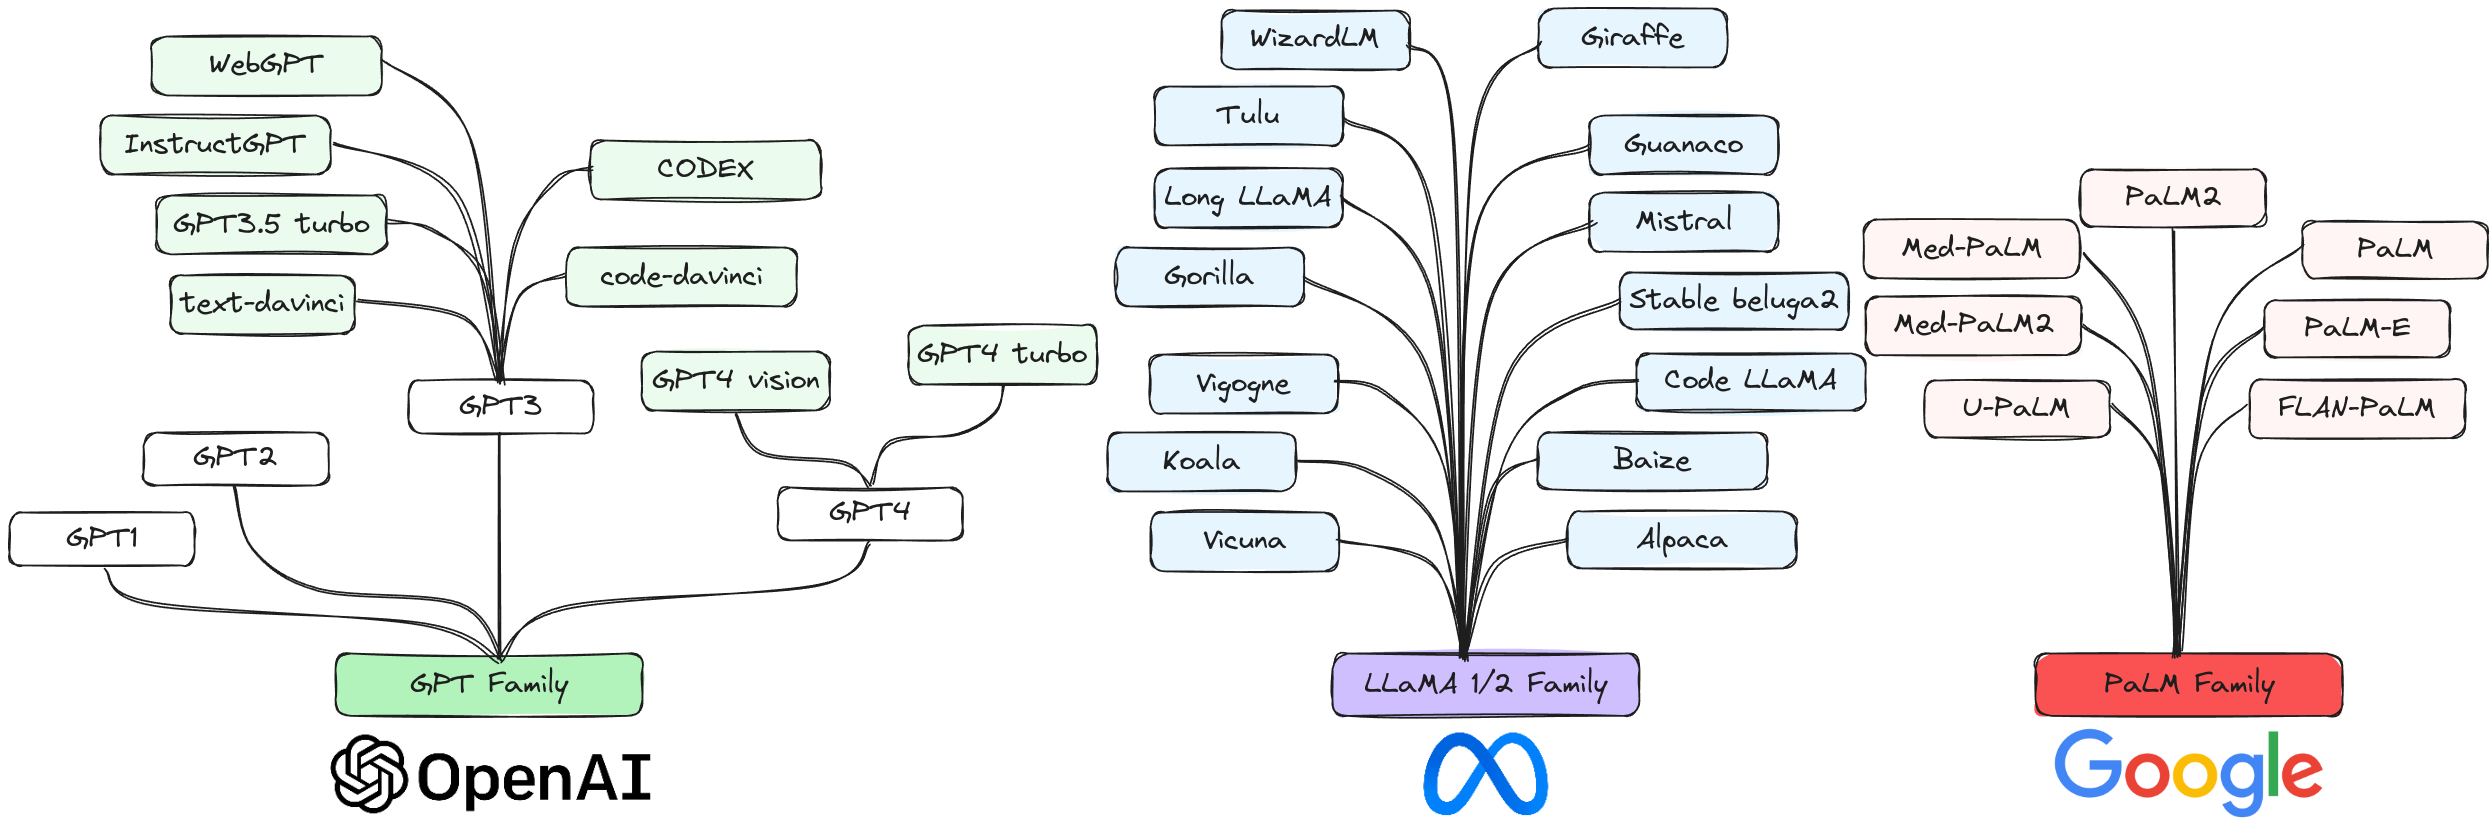
\includegraphics[width=\textwidth,height=6cm,keepaspectratio=true]{llm-families.png}
    \caption{
        \it{Popular LLM families \cite{minaee2024large}}
    }
    \label{fig:llm-families}
\end{figure}

\textbf{The GPT Family:} Generative Pre-trained Transformers (GPT) are a series of decoder-only Transformer-based language models developed by OpenAI. This series includes models such as GPT-1, GPT-2, GPT-3, InstrucGPT, ChatGPT, GPT-4, CODEX, and WebGPT. While the earlier models, such as GPT-1 and GPT-2, are open-source, the more recent models, including GPT-3 and GPT-4, are proprietary and accessible only through APIs.

\textbf{The LLaMA Family:} LLaMA is a series of foundational language models released by Meta. In contrast to GPT models, LLaMA models are open-source, with model weights made available to the research community under a noncommercial license. Consequently, the LLaMA family has expanded rapidly, as these models are widely utilized by numerous research groups to develop improved open-source language models to compete with proprietary models or to create task-specific models for mission-critical applications.

\textbf{The PaLM Family:} The PaLM (Pathways Language Model) family, developed by Google, includes the first PaLM model \cite{chowdhery2022palm} announced in April 2022 and kept private until March 2023. This transformer-based LLM features 540 billion parameters and is pre-trained on a high-quality text corpus containing 780 billion tokens, covering a broad spectrum of natural language tasks and applications. The model's pre-training utilized 6144 TPU v4 chips within the Pathways system, facilitating highly efficient training across multiple TPU Pods. PaLM showcases the ongoing advantages of scaling, achieving state-of-the-art few-shot learning results on hundreds of language understanding and generation benchmarks. The PaLM-540B model not only surpasses state-of-the-art fine-tuned models on various multi-step reasoning tasks but also performs comparably to humans on the newly introduced BIG-bench benchmark.

\subsection{Tokenizations}

Tokenization refers to the process of converting a sequence of text into smaller units known as tokens. While the simplest tokenization tools split text based on whitespace, most rely on a word dictionary. However, this approach faces the out-of-vocabulary (OOV) problem, as the tokenizer can only recognize words present in its dictionary. To address this, popular tokenizers for LLMs are based on sub-words, which can be combined to form a vast array of words, including those not seen in the training data or from different languages. The following sections describe three popular tokenizers \cite{minaee2024large}.

\subsubsection*{BytePairEncoding}

BytePairEncoding (BPE) is originally a data compression algorithm that leverages frequent patterns at the byte level to compress data. The algorithm primarily aims to retain frequent words in their original form while breaking down less common words. This approach ensures that the vocabulary remains manageable in size while adequately representing common words. Additionally, BPE effectively represents morphological variations of frequent words if their suffixes or prefixes are commonly found in the training data.

\subsubsection*{WordPieceEncoding}

This algorithm is predominantly used in well-known models such as BERT and Electra. At the beginning of training, it incorporates the entire alphabet from the training data to ensure that no characters are left as UNK (unknown). This scenario occurs when the model encounters input that cannot be tokenized, typically involving untokenizable characters. Similar to BytePairEncoding, this approach aims to maximize the likelihood of including all tokens in the vocabulary based on their frequency.

\subsubsection*{SentencePieceEncoding}

Although the previously described tokenizers offer significant advantages over white-space tokenization, they still assume that words are always separated by white spaces. This assumption does not hold true for all languages, where words can be disrupted by various noisy elements such as unwanted spaces or invented words. SentencePieceEncoding aims to address this issue.

\subsection{Positional Encoding}

\subsubsection*{Absolute Positional Embeddings}

Absolute Positional Embeddings (APE) \cite{vaswani2023attention} has been used in the original Transformer model to preserve the sequence order information. Consequently, positional information of words is added to the input embeddings at the base of both the encoder and decoder stacks. Various options exist for positional encodings, including learned or fixed methods. In the vanilla Transformer, sine and cosine functions are utilized for this purpose. However, the main drawback of using APE in Transformers is its limitation to a fixed number of tokens. Moreover, APE does not account for the relative distances between tokens.


\subsubsection*{Relative Positional Embeddings}

Relative Positional Embeddings(RPE) \cite{shaw2018selfattention} extend self-attention to consider the pairwise connections between input elements. RPE is integrated into the model at two levels: first, as an additional component to the keys, and subsequently, as a sub-component of the values matrix. This methodology views the input as a fully-connected graph with labels and directed edges. In the context of linear sequences, edges can encode information about the relative positional disparities between input elements. A clipping distance, denoted as \( k^2 \leq k \leq n - 4 \), specifies the maximum limit on relative locations. This mechanism enables the model to make sensible predictions for sequence lengths not present in the training data.

\subsubsection*{Rotary Position Embeddings}

Rotary Positional Embedding (RoPE) \cite{su2023roformer} addresses limitations inherent in existing approaches. Learned absolute positional encodings may lack generalizability and significance, particularly in the context of short sentences. Additionally, current methods such as T5's positional embedding struggle with constructing a complete attention matrix between positions. RoPE employs a rotation matrix to encode the absolute position of words while concurrently incorporating explicit relative position details in self-attention. This approach offers several advantageous features, including flexibility with varying sentence lengths, reduced word dependency as relative distances increase, and enhancement of linear self-attention through relative position encoding. Notably, models like GPT-NeoX-20B, PaLM, CODEGEN, and LLaMA leverage RoPE within their architectures.

\subsubsection*{Relative Positional Bias}

The rationale behind this form of positional embedding is to enable extrapolation during inference for sequences longer than those encountered during training. In their work \cite{press2022train}, Press et al. introduced Attention with Linear Biases (ALiBi). Rather than solely adding positional embeddings to word embeddings, they introduced a bias to the attention scores of query-key pairs, imposing a penalty proportional to their distance. The BLOOM \cite{workshop2023bloom} model leverages ALiBi as part of its architecture.

\begin{figure}[H]
    \centering

    \begin{subfigure}[b]{.49\linewidth}
        \centering
        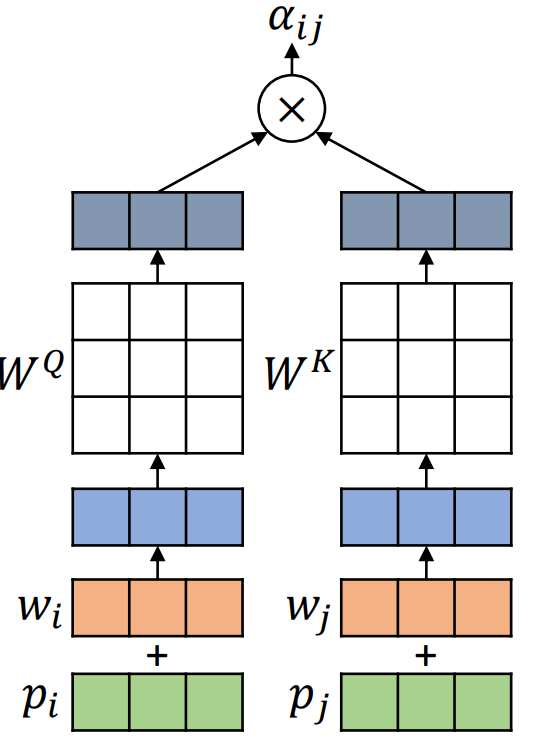
\includegraphics[width=\textwidth,height=6cm,keepaspectratio=true]{ape.png}
        \caption{
            \it{Absolute positional encoding \cite{ke2021rethinking}}
        }
    \end{subfigure}
    \hfill
    \begin{subfigure}[b]{.49\linewidth}
        \centering
        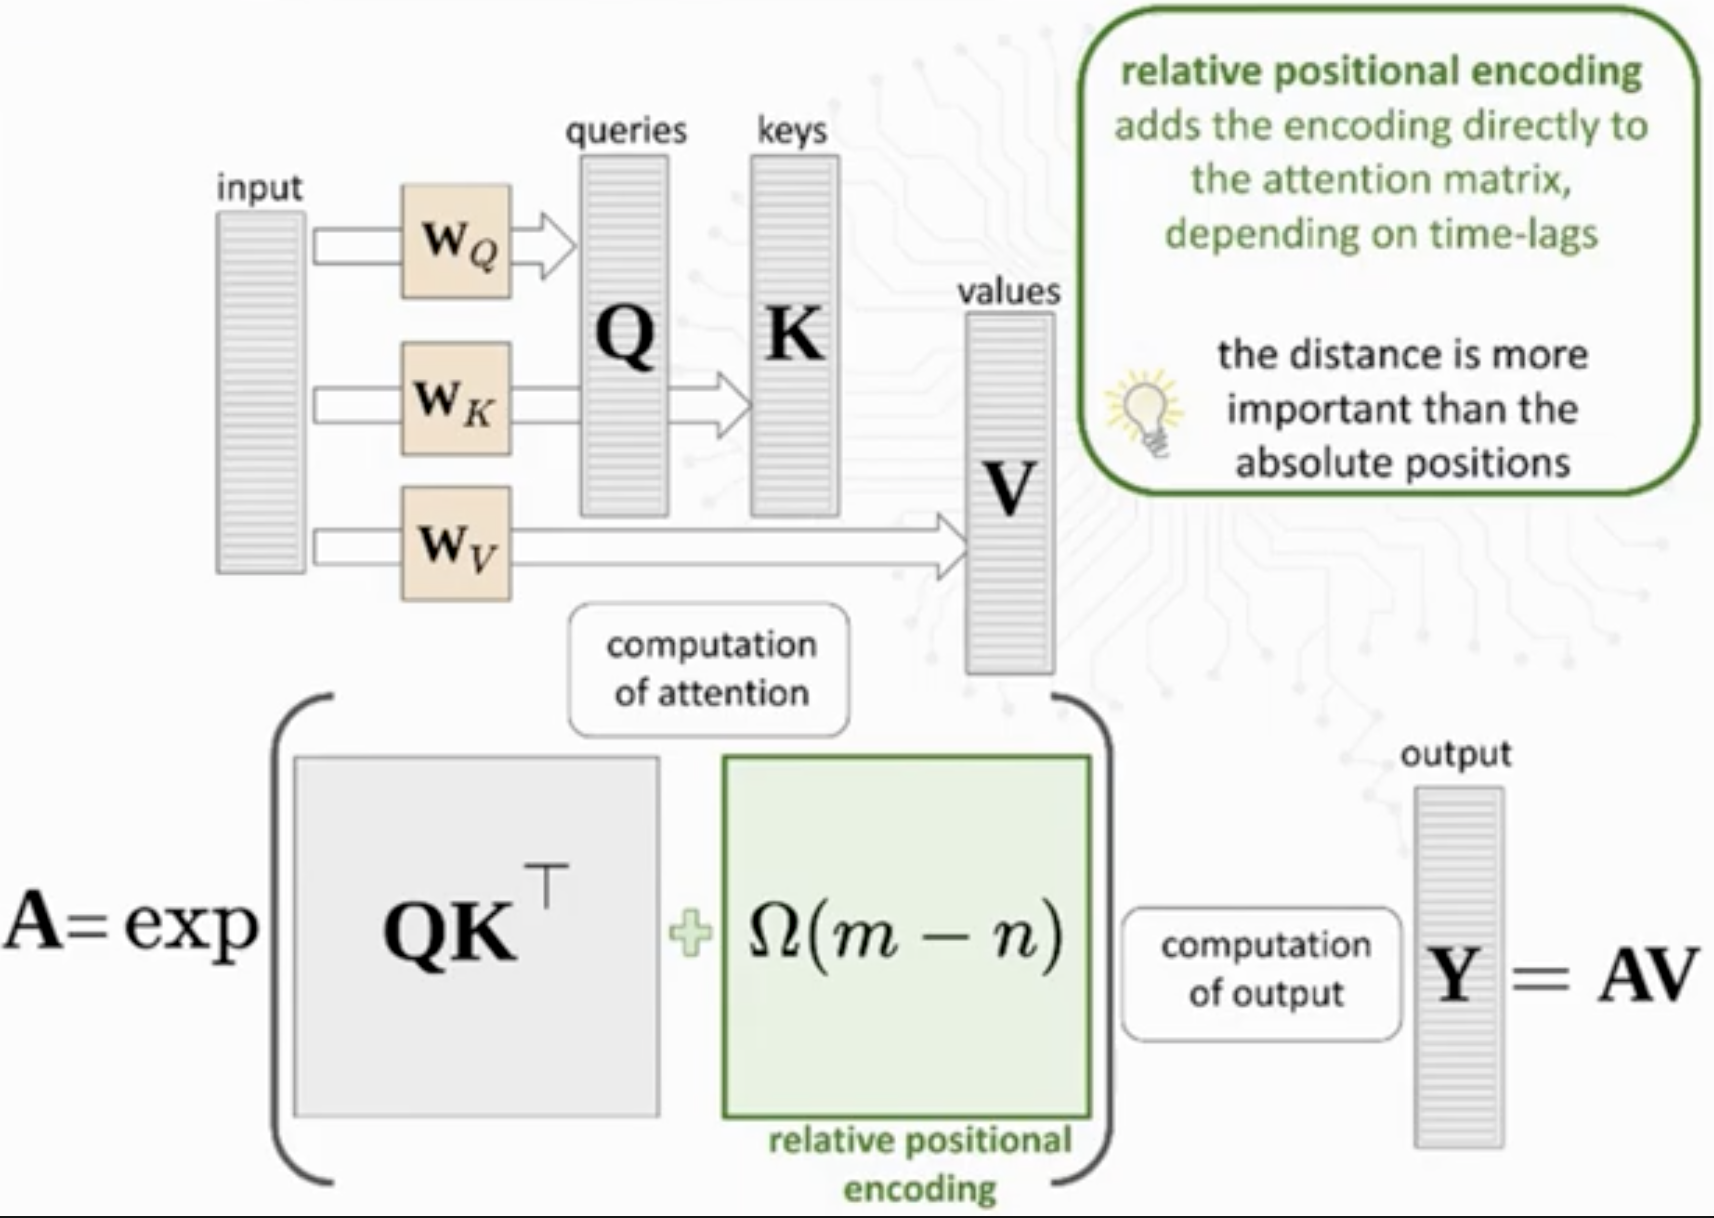
\includegraphics[width=\textwidth,height=6cm,keepaspectratio=true]{rpe.png}
        \caption{
            \it{Relative Positional Embeddings}
        }
    \end{subfigure}
    \par\bigskip
    \begin{subfigure}[b]{.49\linewidth}
        \centering
        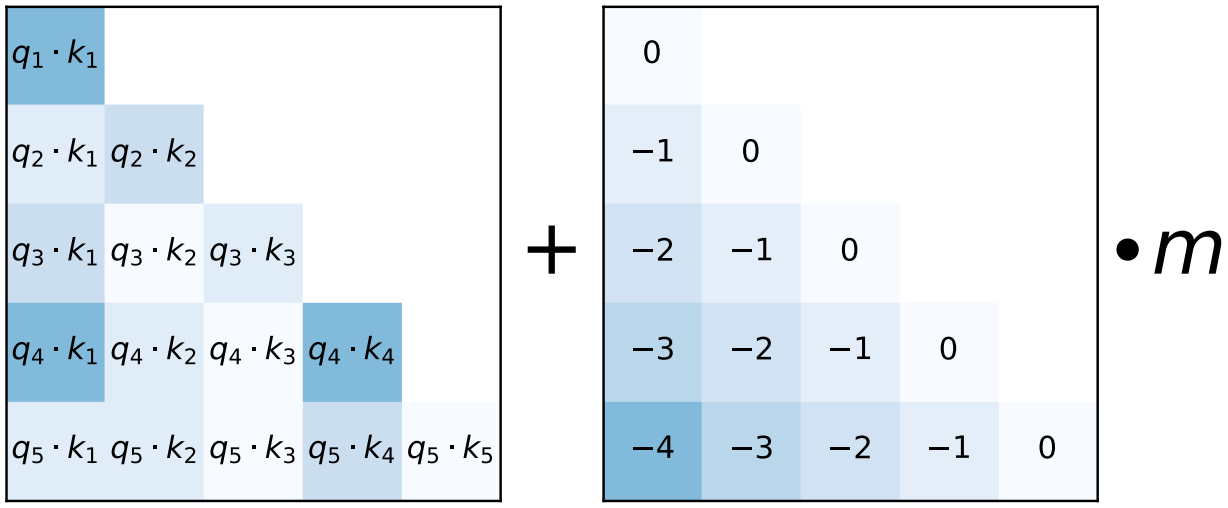
\includegraphics[width=\textwidth,height=6cm,keepaspectratio=true]{alibi.png}
        \caption{
            \it{Relative Positional Bias \cite{press2022train}}
        }
    \end{subfigure}
    \hfill
    \begin{subfigure}[b]{.49\linewidth}
        \centering
        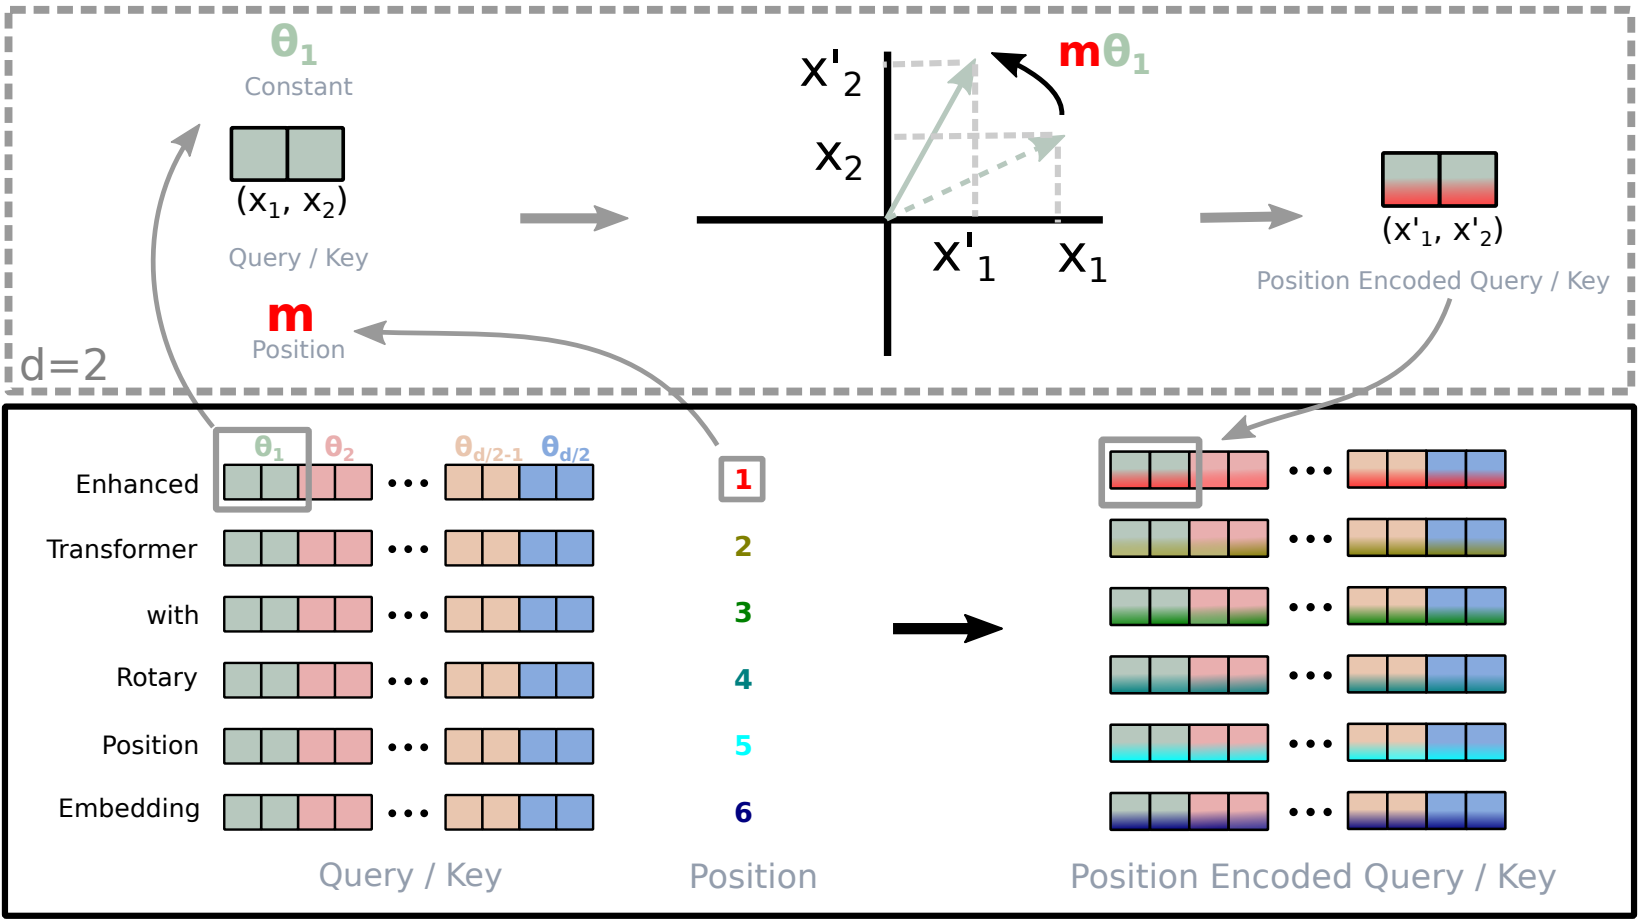
\includegraphics[width=\textwidth,height=6cm,keepaspectratio=true]{rope.png}
        \caption{
            \it{Rotary Positional Embedding \cite{su2023roformer}}
        }
    \end{subfigure}

    \caption{\it{Various positional encodings employed in LLMs}}

\end{figure}

\subsection{Model Pre-training}

Pre-training is the very first step in the large language model training pipeline, helping LLMs acquire fundamental language understanding capabilities, which can be useful in a wide range of language-related tasks. During pre-training, the LLM is trained on a massive amount of (usually) unlabeled texts, typically in a self-supervised manner. There are different approaches used for pre-training, such as next sentence prediction \cite{devlin2019bert}. The two most common techniques include next token prediction (autoregressive language modeling) and masked language modeling.

In the \textbf{Autoregressive Language Modeling} framework, given a sequence of n tokens \( x_1, \ldots, x_n \), the model aims to predict the next token \( x_{n+1} \) (and occasionally the subsequent sequence of tokens) in an autoregressive manner. A commonly used loss function in this context is the log-likelihood of the predicted tokens, as demonstrated in Equation \ref{eq:alm}.

\begin{equation}\label{eq:alm}
    \mathcal{L}_{ALM}(x) = \sum_{i=1}^N p(x_{i+n} |x_i, \ldots, x_{i+n-1})
\end{equation}

Given the autoregressive nature of this framework, decoder-only models are inherently better suited to learn and perform these tasks.

\hfill

In \textbf{Masked Language Modeling}, certain words in a sequence are masked, and the model is trained to predict these masked words based on the surrounding context. This approach is sometimes referred to as denoising autoencoding. If we denote the masked or corrupted samples in the sequence \( x \) as \( \tilde{x} \), the training objective can be expressed as:


\begin{equation}
    \mathcal{L}_{MLM}(x) = \sum_{i=1}^N p(\tilde{x}|x\backslash \tilde{x})
\end{equation}

\hfill

More recently, \textbf{Mixture of Experts (MoE)} \cite{shazeer2017outrageously}, \cite{fedus2022switch} have gained significant popularity in the LLM space. MoEs allow models to be pre-trained with substantially less compute, enabling a dramatic increase in model or dataset size within the same compute budget as a dense model. An MoE architecture consists of two main components: Sparse MoE layers, which replace dense feed-forward network (FFN) layers, and contain several "experts" (e.g., 8), each of which is a neural network. Typically, these experts are FFNs, but they can also be more complex networks. A gate network, or router, determines which tokens are sent to which expert. Notably, a token can be routed to multiple experts. Routing tokens to experts is a critical decision in MoE design; the router consists of learned parameters and is trained concurrently with the rest of the network. Figure 29 illustrates a Switch Transformer encoder block, commonly used in MoEs.


\begin{figure}[H]
    \centering
    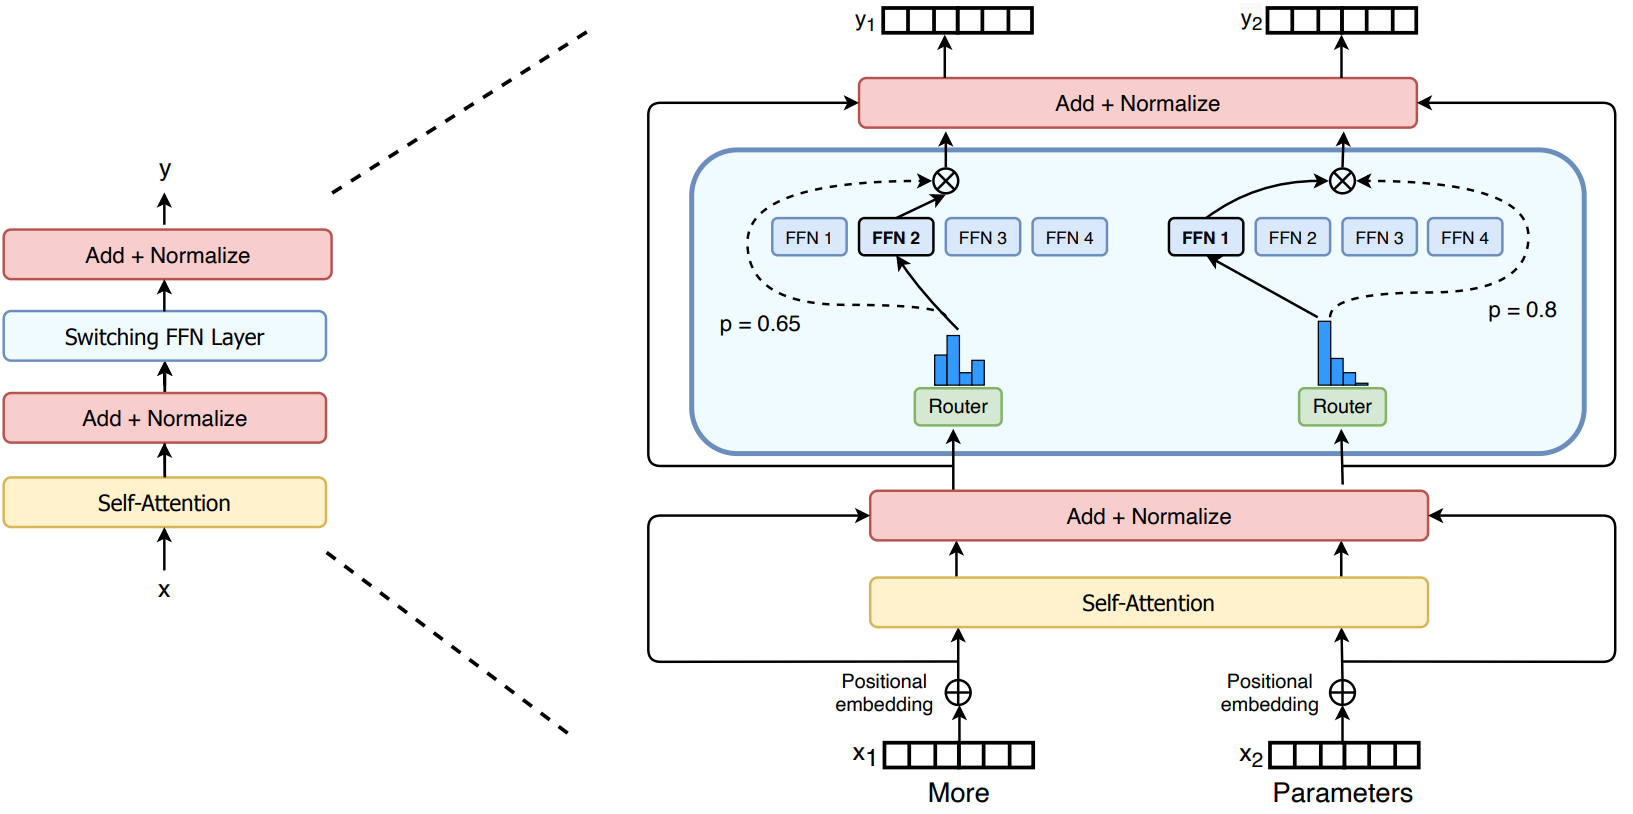
\includegraphics[width=\textwidth,height=6cm,keepaspectratio=true]{moe.png}
    \caption{
        \it{Illustration of a Switch Transformer encoder block.
            They replaced the dense feed forward network (FFN) layer present in the Transformer with a sparse Switch FFN layer
            (light blue). \cite{fedus2022switch}}
    }
    \label{fig:moe}
\end{figure}


\subsection{Fine-tuning and Instruction Tuning}

Early language models, such as BERT, trained using self-supervision, were not able to perform specific tasks directly. To make the foundation model useful, it needed to be fine-tuned for a specific task using labeled data, a process known as supervised fine-tuning (SFT). For instance, in the original BERT paper \cite{devlin2019bert}, the model was fine-tuned for 11 different tasks. While more recent LLMs no longer require fine-tuning to be functional, they can still benefit from task-specific or data-specific fine-tuning. For example, OpenAI reports that the much smaller GPT-3.5 Turbo model can outperform GPT-4 when fine-tuned with task-specific data\footnote{\url{https://platform.openai.com/docs/guides/fine-tuning}}.

Fine-tuning does not have to be limited to a single task; various approaches to multi-task fine-tuning exist (see, e.g., Mahabi et al. \cite{mahabadi2021parameterefficient}). Fine-tuning on one or more tasks is known to improve results and reduce the complexity of prompt engineering, offering an alternative to retrieval-augmented generation. Additionally, there are other compelling reasons to fine-tune a model. For instance, fine-tuning can expose the model to new or proprietary data that it did not encounter during pre-training.

An essential motivation for fine-tuning LLMs is to ensure that their responses align with the expectations humans have when providing instructions through prompts. This process is referred to as instruction tuning \cite{zhang2024instruction}. While we delve into the specifics of designing and engineering prompts in later sections, it's crucial to grasp that in the context of instruction tuning, the instruction acts as a prompt that outlines the task the LLM is expected to perform. Instruction tuning datasets, such as Natural Instructions \cite{mishra2022crosstask}, encompass not only the task definition but also include other components such as positive and negative examples or instructions on what to avoid.

The specific methodology and instruction datasets utilized for instruction tuning an LLM may vary; however, as a general trend, instruction-tuned models tend to surpass the performance of their original foundation models upon which they are built. For instance, InstructGPT \cite{ouyang2022training} exhibits superior performance to GPT-3 across most benchmarks. Similarly, Alpaca \cite{alpaca} outperforms LLaMA in comparative evaluations.

\textbf{Self-Instruct} \cite{wang2023selfinstruct}, introduced by Wang et al., is another prominent method in this domain. They proposed a framework aimed at enhancing the instruction-following abilities of pre-trained language models by leveraging their own generated outputs. Their pipeline involves generating instructions, input, and output samples from a language model, followed by filtering out invalid or redundant ones before employing them to fine-tune the original model.

\subsection{Reinforcement Learning from Human Feedback (RLHF)}

AI Alignment is the process of steering AI systems towards human goals, preferences, and principles. LLMs, pre-trained for word prediction, often exhibit unintended behaviors. For example, they might generate contents that are toxic, harmful, misleading and biased.

Instruction tuning, discussed above, gets LLMs a step closer to being aligned. However, in many cases, it is important to include further steps to improve the alignment of the model and avoid unintended behaviors.

Reinforcement Learning from Human Feedback (RLHF) is a powerful technique used to fine-tune large language models (LLMs) by leveraging human-generated feedback. This approach helps address limitations of supervised fine-tuning, such as overfitting to the training data, and enables LLMs to better align with human preferences and values. This section explores the key components and process of RLHF \cite{christiano2023deep}.

\subsubsection*{Collecting Human Feedback}

The first step in RLHF involves collecting human feedback on model-generated outputs. This can be achieved through several methods, such as:

\begin{itemize}
    \item Providing demonstrations of correct behavior.
    \item Comparing different model-generated outputs and ranking them based on quality.
    \item Assigning explicit rewards or scores to model outputs.
\end{itemize}

The collected feedback serves as a valuable source of information for the model to learn from, helping it better understand human preferences and expectations.

\subsubsection*{Reward Modeling}

Once human feedback is collected, a reward model is trained to predict the quality of the model-generated outputs. This reward model acts as a proxy for human judgment and is used to guide the reinforcement learning process. By training the reward model on human-generated feedback, it learns to approximate human preferences and assign rewards accordingly.

\subsubsection*{Reinforcement Learning}

With a reward model in place, the LLM is fine-tuned using reinforcement learning algorithms such as Proximal Policy Optimization (PPO) \cite{schulman2017proximal} or REINFORCE \cite{ahmadian2024basics}. The goal is to generate outputs that maximize the predicted rewards, which are a proxy for human preferences. By optimizing the model's behavior to align with the reward model, LLMs can learn to generate outputs that are more desirable and useful to human users.

\subsubsection*{Iterative Improvement}

The RLHF process is iterative. As the model improves, additional human feedback can be collected to further refine the reward model. This updated reward model is then used to guide another round of reinforcement learning, resulting in continued performance improvements.

Through these iterations, LLMs can learn to better align with human values and preferences, which can lead to higher-quality outputs and improved performance on specific tasks. RLHF has been successfully applied to fine-tune models like OpenAI's ChatGPT \cite{ouyang2022training}, demonstrating its effectiveness in enhancing the capabilities of LLMs.

\subsection{How LLMs are used and augmented}

Once LLMs are trained, they become capable of generating desired outputs for various tasks. While LLMs can be directly utilized through basic prompting, fully exploiting their potential or overcoming some of their limitations often requires augmentation through external means. In this section, we initially provide a concise overview of the primary shortcomings of LLMs, with a particular focus on the issue of hallucination. We then discuss how prompting and certain augmentation strategies can not only mitigate these limitations but also enhance the capabilities of LLMs, potentially transforming them into comprehensive AI agents with the capacity to interact with the external world.

\subsubsection*{LLM limitations}

It's crucial to acknowledge that LLMs are trained to predict tokens. Despite the enhancements brought about by fine-tuning and alignment, they still exhibit significant limitations, especially if used in a simplistic manner. Some notable constraints include:

\begin{itemize}
    \item Lack of state/memory: LLMs inherently lack the ability to retain information from previous prompts, which poses a challenge for tasks requiring some form of state management.
    \item Stochastic/probabilistic nature: Repeatedly sending the same prompt to an LLM may result in different responses due to its probabilistic nature. Although parameters like temperature can mitigate variability, this trait stems from their training process and can lead to inconsistent outputs.
    \item Limited access to external data: LLMs operate in isolation and lack real-time information or access to data beyond their training set.
    \item Large resource requirements: Given their substantial size, training and serving LLMs often necessitate expensive GPU resources. Larger models may also exhibit poor service level agreements (SLAs), particularly concerning latency.
    \item Hallucinatory tendencies: LLMs lack a definitive concept of "truth" and have been trained on diverse content, leading to the generation of plausible yet inaccurate responses.
\end{itemize}

While all these limitations are pertinent to various applications, it's particularly insightful to delve deeper into the issue of hallucinations. This phenomenon has garnered significant attention in recent months and has catalyzed the development of numerous prompting approaches and LLM augmentation techniques, as we'll explore further.

\hfill

In the domain of Large Language Models (LLMs), the concept of \textbf{"hallucinations"} has become a focal point of discussion. Defined in the literature, particularly in the paper "Survey of Hallucination in Natural Language Generation" \cite{Ji_2023}, hallucination within an LLM refers to "the generation of content that is nonsensical or deviates from the provided source." Although the term originates from psychological discourse, it has been adopted and adapted within the realm of artificial intelligence.

Hallucinations in LLMs can be broadly categorized into
two types:

\begin{enumerate}
    \item \textbf{Intrinsic Hallucinations:} These directly conflict with the source material, introducing factual inaccuracies or logical inconsistencies.
    \item \textbf{Extrinsic Hallucinations:} These, while not contradicting, are unverifiable against the source, encompassing speculative or unconfirmable elements.
\end{enumerate}

In LLM contexts, the definition of 'source' varies depending on the task at hand. In dialogue-based tasks, 'source' typically refers to 'world knowledge,' encompassing a broad range of factual and contextual information. Conversely, in tasks like text summarization, the 'source' is more narrowly defined as the input text itself. This distinction holds significance in assessing and understanding hallucinations within LLM-generated content. Furthermore, the implications of hallucinations are highly context-dependent. For instance, in creative endeavors such as poem writing, hallucinations may be considered acceptable or even advantageous, as they can contribute to artistic expression and innovation.

LLMs, trained on diverse datasets sourced from the internet, books, and Wikipedia, generate text based on probabilistic models, lacking an intrinsic understanding of truth or falsehood. Despite recent advancements such as instruct tuning and Reinforcement Learning from Human Feedback (RLHF), which aim to guide LLMs toward producing more factually accurate outputs, the fundamental probabilistic nature and associated limitations persist. A recent study titled "Sources of Hallucination by Large Language Models on Inference Tasks" \cite{mckenna2023sources} sheds light on two critical factors contributing to hallucinations in LLMs: the veracity prior and the relative frequency heuristic. This underscores the intricate challenges involved in LLM training and output generation.

\begin{figure}[H]
    \centering
    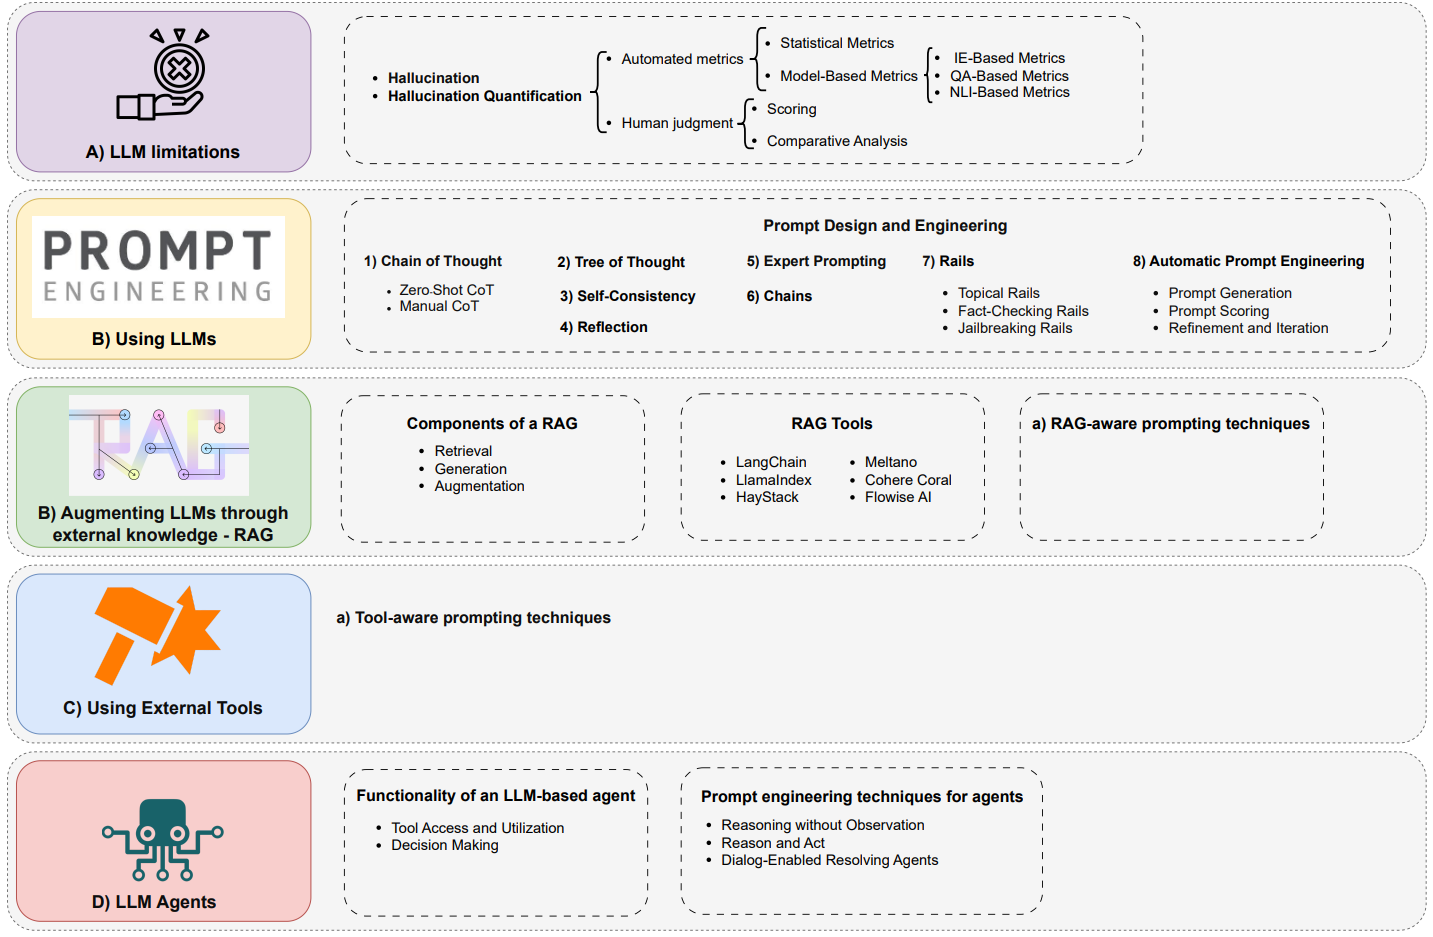
\includegraphics[width=\textwidth,height=8cm,keepaspectratio=true]{llms-used-and-augmented.png}
    \caption{
        \it{How LLMs Are Used and Augmented \cite{minaee2024large}.}
    }
    \label{fig:llm-used-and-augmented}
\end{figure}

\subsubsection*{Prompt Design and Engineering}

In generative AI models, a prompt refers to the textual input provided by users to steer the model's output. This input can vary from straightforward questions to detailed descriptions or specific tasks. Typically, prompts encompass instructions, questions, input data, and examples. In practice, to prompt a desired response from an AI model, a prompt must include either instructions or questions, although other elements are optional. Advanced prompts may involve more intricate structures, such as "chain of thought" prompting, where the model is directed to follow a logical reasoning process to generate an answer.

Prompt engineering is a rapidly evolving discipline that shapes the interactions and outputs of LLMs and other generative AI models. At its core, prompt engineering involves crafting optimal prompts to achieve specific goals with a generative model. This process goes beyond merely instructing the model; it also requires a deep understanding of the model's capabilities and limitations, as well as the context in which it operates.

Researchers employ prompt engineering to enhance the performance of LLMs across a broad spectrum of tasks, including question answering and arithmetic reasoning. Developers utilize prompt engineering to create robust and effective prompting techniques that interface seamlessly with LLMs and other tools.

Prompt engineering extends beyond the design and development of prompts. It encompasses a wide array of skills and techniques essential for interacting with and developing LLMs. This discipline is crucial for interfacing with LLMs, building applications with them, and understanding their capabilities. Through prompt engineering, one can enhance the safety of LLMs and develop new functionalities, such as augmenting LLMs with domain knowledge and integrating external tools.

In the following paragraphs we detail some of the most
interesting and popular prompt engineering approaches.

\hfill

1) Chain of Thought (CoT): The Chain of Thought (CoT) technique, first described in the paper "Chain-of-Thought Prompting Elicits Reasoning in Large Language Models" \cite{wei2023chainofthought} by Google researchers, marks a significant advancement in prompt engineering for Large Language Models (LLMs). This method is based on the understanding that although LLMs excel in token prediction, they are not inherently designed for explicit reasoning. CoT mitigates this limitation by guiding the model through essential reasoning steps.

\begin{figure}[H]
    \centering
    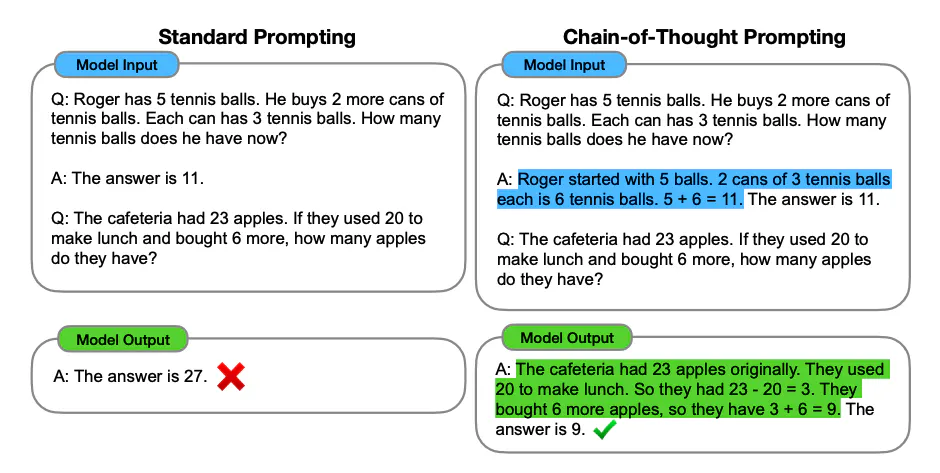
\includegraphics[width=\textwidth,height=8cm,keepaspectratio=true]{cot.png}
    \caption{
        \it{Chain-of-Thought (CoT) Prompting \cite{wei2023chainofthought}}
    }
\end{figure}

CoT is designed to make the implicit reasoning process of LLMs explicit. By outlining the necessary reasoning steps, this technique guides the model towards producing more logical and reasoned outputs, particularly in scenarios that demand more than simple information retrieval or pattern recognition.

\hfill

2) Tree of Thought (ToT): The Tree of Thought (ToT) prompting technique \cite{yao2023tree} draws inspiration from the concept of exploring various alternative solutions or thought processes before settling on the most plausible one. ToT involves branching out into multiple "thought trees," with each branch representing a different line of reasoning. This method enables the LLM to investigate various possibilities and hypotheses, mirroring human cognitive processes where multiple scenarios are considered before determining the most likely outcome.


A critical aspect of ToT is the evaluation of these reasoning paths. As the LLM generates different branches of thought, each branch is assessed for its validity and relevance to the query. This process involves real-time analysis and comparison of the branches, ultimately leading to the selection of the most coherent and logical outcome.

ToT is particularly useful in complex problem-solving scenarios where a single line of reasoning might not suffice. It enables LLMs to mimic a more human-like problem-solving approach by considering a range of possibilities before arriving at a conclusion. This technique enhances the model's ability to handle ambiguity, complexity, and nuanced tasks, making it a valuable tool in advanced AI applications.

\begin{figure}[H]
    \centering
    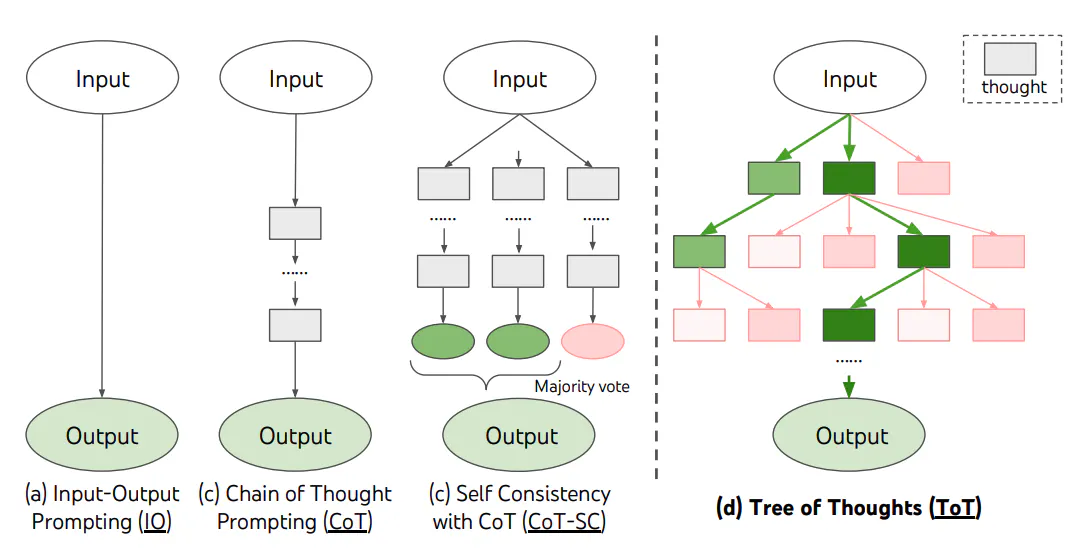
\includegraphics[width=\textwidth,height=8cm,keepaspectratio=true]{tot.png}
    \caption{
        \it{Tree-of-Thought (ToT) Framework \cite{yao2023tree}}
    }
\end{figure}

\hfill

3) Self-Consistency: Self-Consistency \cite{manakul2023selfcheckgpt} employs an ensemble-based method, prompting the LLM to generate multiple responses to the same query. The consistency among these responses acts as an indicator of their accuracy and reliability.

The Self-Consistency approach is based on the principle that if an LLM generates multiple similar responses to the same prompt, the response is more likely to be accurate. This method involves prompting the LLM to address a query multiple times and then analyzing the responses for consistency. This technique is particularly useful in scenarios where factual accuracy and precision are critical.

The consistency of responses can be measured using various methods. One common approach is to analyze the overlap in the content of the responses. Other methods include comparing the semantic similarity of responses or employing more sophisticated techniques like BERT-scores or n-gram overlaps. These measures help quantify the level of agreement among the responses generated by the LLM.

\hfill

4) Reflexion: Reflexion \cite{shinn2023reflexion} involves prompting LLMs to assess and potentially revise their own outputs by reasoning about the correctness and coherence of their responses. The concept of Reflexion centers on the ability of LLMs to engage in a form of self-evaluation. After generating an initial response, the model is prompted to reflect on its own output, considering factors such as factual accuracy, logical consistency, and relevance. This introspective process can lead to the generation of revised or improved responses.

\begin{figure}[H]
    \centering
    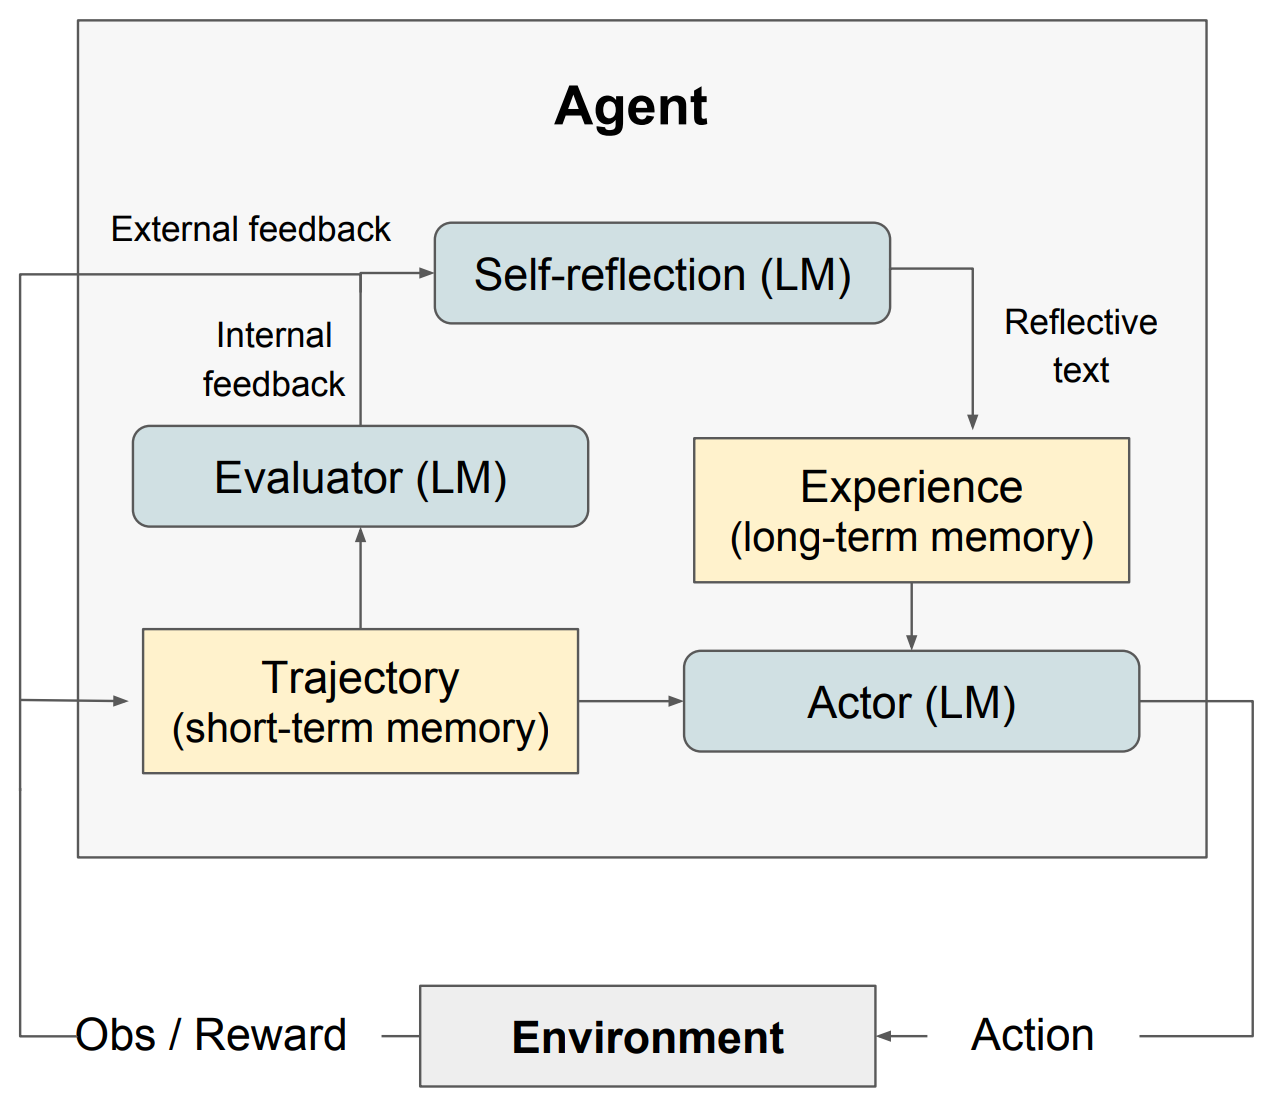
\includegraphics[width=\textwidth,height=8cm,keepaspectratio=true]{reflexion.png}
    \caption{
        \it{Diagram of Reflection \cite{shinn2023reflexion}.}
    }
\end{figure}

A crucial component of Reflexion is the LLM's ability to self-edit. By assessing its initial response, the model can detect potential errors or areas that need improvement. This iterative process of generating, reflecting, and revising enables the LLM to enhance its output, improving the overall quality and reliability of its responses.

\hfill

5) Chains: Chains refer to the method of linking multiple components in a sequence to manage complex tasks with Large Language Models (LLMs). This approach involves creating a series of interconnected steps or processes, each contributing to the final outcome. The concept of Chains is based on constructing a workflow where different stages or components are sequentially arranged. Each component in a Chain performs a specific function, with the output of one serving as the input for the next. This end-to-end arrangement allows for more intricate and nuanced processing, as each stage can be customized to handle a specific aspect of the task. The complexity and structure of Chains can vary based on the requirements. In "PromptChainer: Chaining Large Language Model Prompts through Visual Programming" \cite{wu2022promptchainer}, the authors discuss the main challenges in designing chains and introduce a visual tool to support these tasks.

\begin{figure}[H]
    \centering
    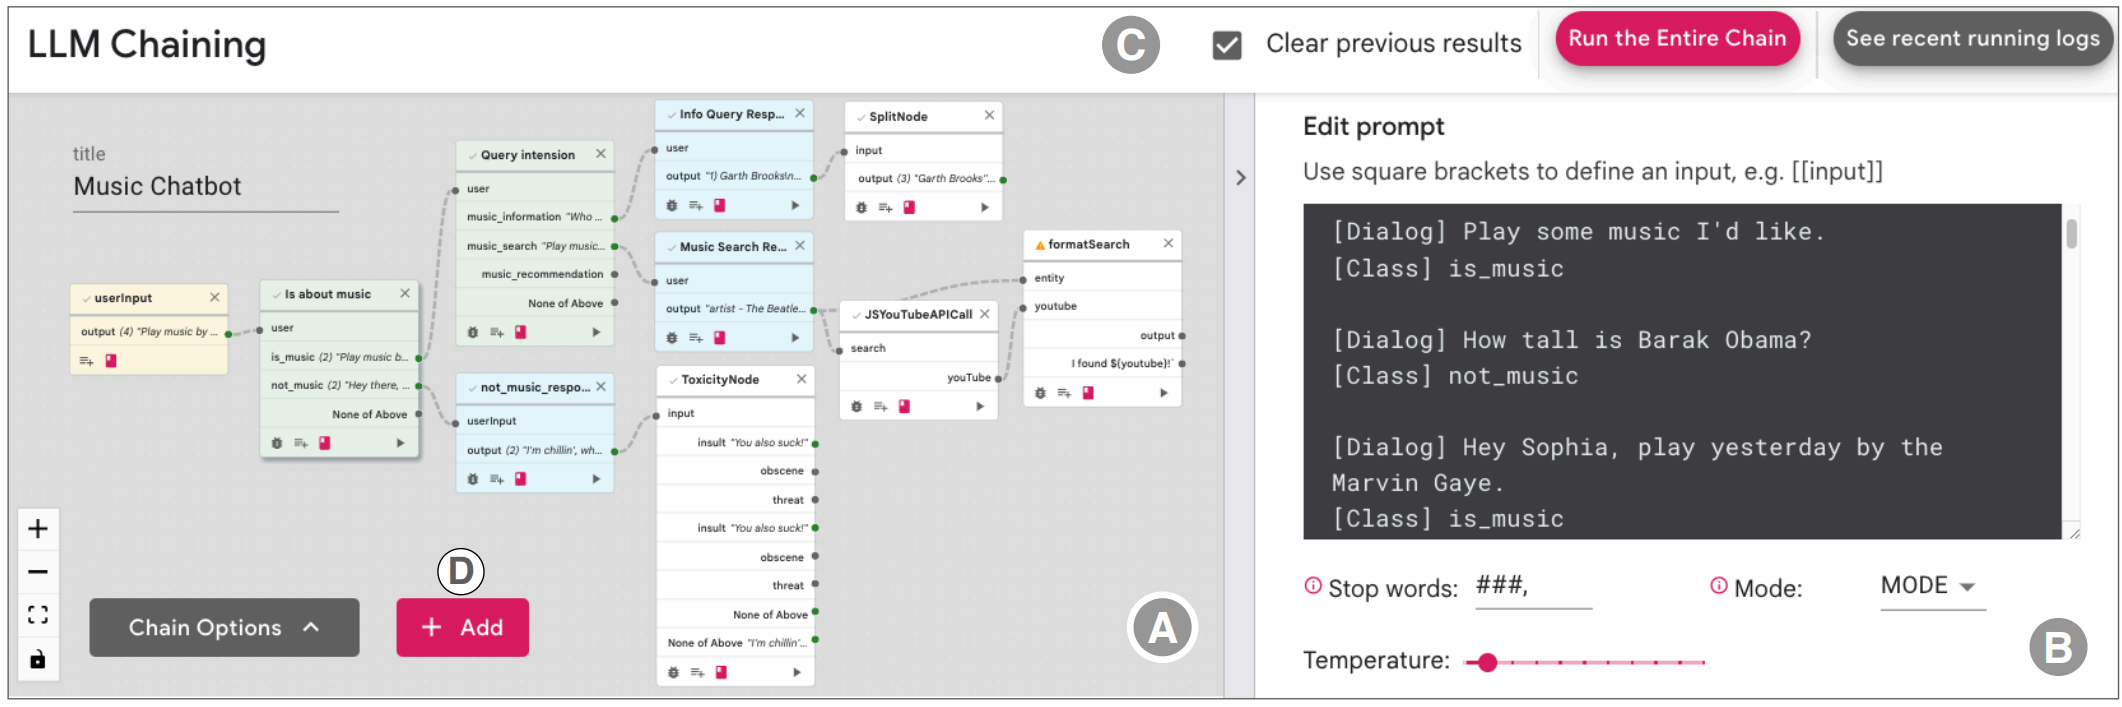
\includegraphics[width=\textwidth,height=8cm,keepaspectratio=true]{chains.png}
    \caption[        \it{The PromptChainer interface.}
    ]{\it{The PromptChainer interface. (A) The Chain View visualizes the chain structure with node-edge diagrams (enlarged
            in Figure 2), and allows users to edit the chain by adding, removing, or reconnecting nodes. (B) The Node View supports implementing, improving, and testing each individual node, e.g., editing prompts for LLM nodes. PromptChainer also supports
            running the chain end-to-end (C) \cite{wu2022promptchainer}.}}
\end{figure}

\hfill

6) Automatic Prompt Engineering (APE): Automatic Prompt Engineering (APE) \cite{zhou2023large} aims to automate the creation of prompts for Large Language Models (LLMs). APE seeks to streamline and optimize the prompt design process by leveraging the capabilities of LLMs themselves to generate and evaluate prompts. This approach involves using LLMs in a self-referential manner, where the model generates, scores, and refines prompts. By recursively utilizing LLMs in this way, APE facilitates the creation of high-quality prompts that are more likely to elicit the desired response or outcome.

\begin{figure}[H]
    \centering
    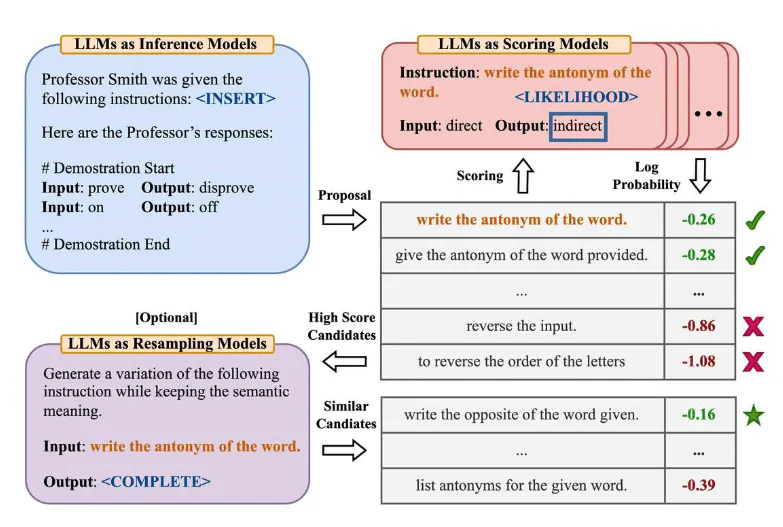
\includegraphics[width=\textwidth,height=8cm,keepaspectratio=true]{apen.png}
    \caption{\it{Automatic Prompt Engineer framework \cite{zhou2023large}.}}
\end{figure}

\subsubsection*{Augmenting LLMs through external knowledge - RAG}

One of the primary limitations of pre-trained Large Language Models (LLMs) is their lack of up-to-date knowledge or access to private or use case-specific information. This is where Retrieval Augmented Generation (RAG) comes into the picture \cite{lewis2021retrievalaugmented}. As illustrated in Figure \ref{fig:rag1}, RAG involves extracting a query from the input prompt and using that query to retrieve relevant information from an external knowledge source (e.g., a search engine or a knowledge graph.). The relevant information is then added to the original prompt and fed to the LLM to generate the final response. A RAG system includes three important components: Retrieval, Generation, and Augmentation \cite{gao2024retrievalaugmented}.

\begin{figure}[H]
    \centering
    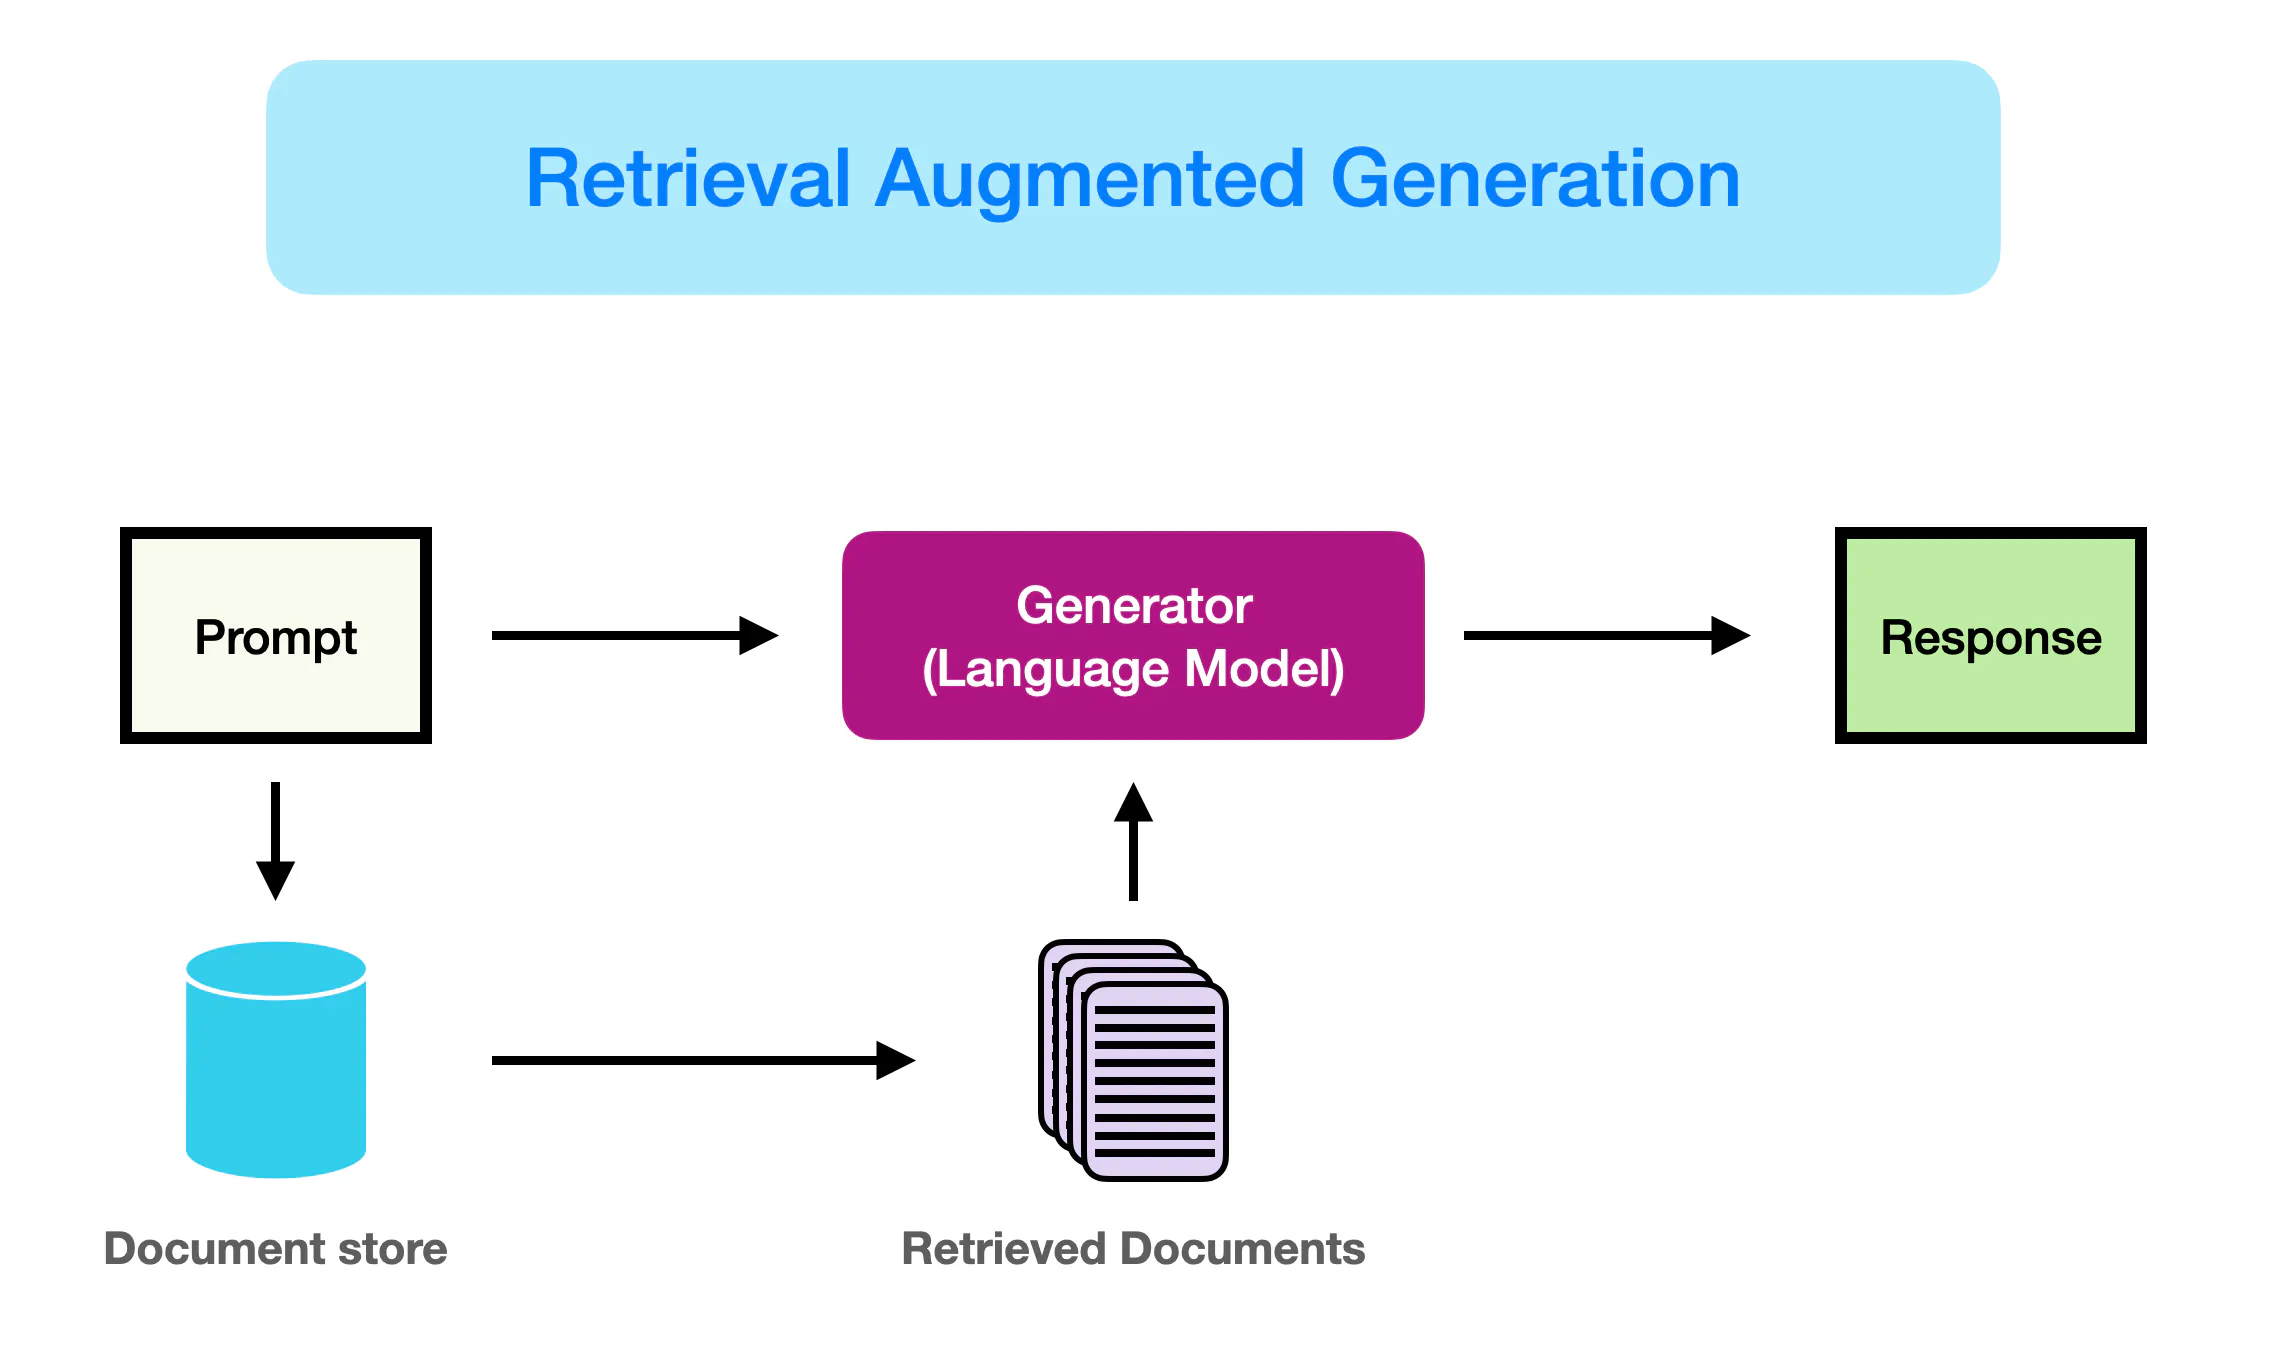
\includegraphics[width=\textwidth,height=8cm,keepaspectratio=true]{rag.png}
    \caption{\it{An example of synthesizing RAG with LLMs for question answering application.}}
    \label{fig:rag1}
\end{figure}

Due to the significance of RAG in the development of advanced LLM systems, several RAG-aware prompting techniques have been developed recently. One such technique is Forward-looking Active Retrieval Augmented Generation (FLARE).

Forward-looking Active Retrieval Augmented Generation (FLARE) \cite{jiang2023active} enhances the capabilities of Large Language Models (LLMs) by iteratively integrating prediction and information retrieval. FLARE represents an advancement in retrieval-augmented generation, aimed at improving the accuracy and relevance of LLM responses.

FLARE involves an iterative process where the LLM actively predicts upcoming content and uses these predictions as queries to retrieve relevant information. This method differs from traditional retrieval-augmented models, which typically retrieve information once before proceeding with generation. In FLARE, the process is dynamic and ongoing throughout the generation phase. Each sentence or segment generated by the LLM is evaluated for confidence. If the confidence level falls below a certain threshold, the model uses the generated content as a query to retrieve relevant information, which is then used to regenerate or refine the sentence. This iterative process ensures that each part of the response is informed by the most relevant and current information available.